\subsection{The Schwarzian Derivative}

In this example we will derive the form of the Schwarzian derivative \(Su\) for a smooth function \(u:\mathbb R \to \mathbb R\)
given by
\begin{equation}
Su = \frac{u'''}{u'} - \frac{3}{2}\left(\frac{u''}{u'}\right)^2.
\end{equation}
What is special about the Schwarzian derivative is that you get the same result if you apply it to
a function \(w\) that is a linear fractional transformation of \(f\), i.e. for
\begin{equation}
w(x) = \frac{A + Bu(x)}{C + Du(x)},
\end{equation}
for constants \(A, B, C,\) and \(D\), we have that \(Su = Sw\). We will first briefly discuss 
linear fractional transformations and then how we aim to derive the Schwarzian derivative from the
above invariance property.

\subsubsection*{The Setup: Linear Fractional Transformations}

A linear fractional transformation for one real variable is a function of the form
\begin{equation}
T(y) = \frac{A + By}{C + Dy},
\end{equation}
for constants \(A, B, C\) and \(D\). Note that the function is not defined for the single point \(C + Dy = 0\) when
\(D\neq 0\).

An important motivation for linear fractional transformations is perspective transformations. First imagine an
eye sitting at the origin in \(\mathbb R^2\), and the eye is looking down the x-axis towards \(+\infty\). 
Everything the eye
observes is equivalent to seeing something sitting in its viewing line (or plane for 3-dimensions). We will
take the viewing line of the eye to be \(\{x = 1\}\). See the figure below.

\begin{figure}[h]
\centering
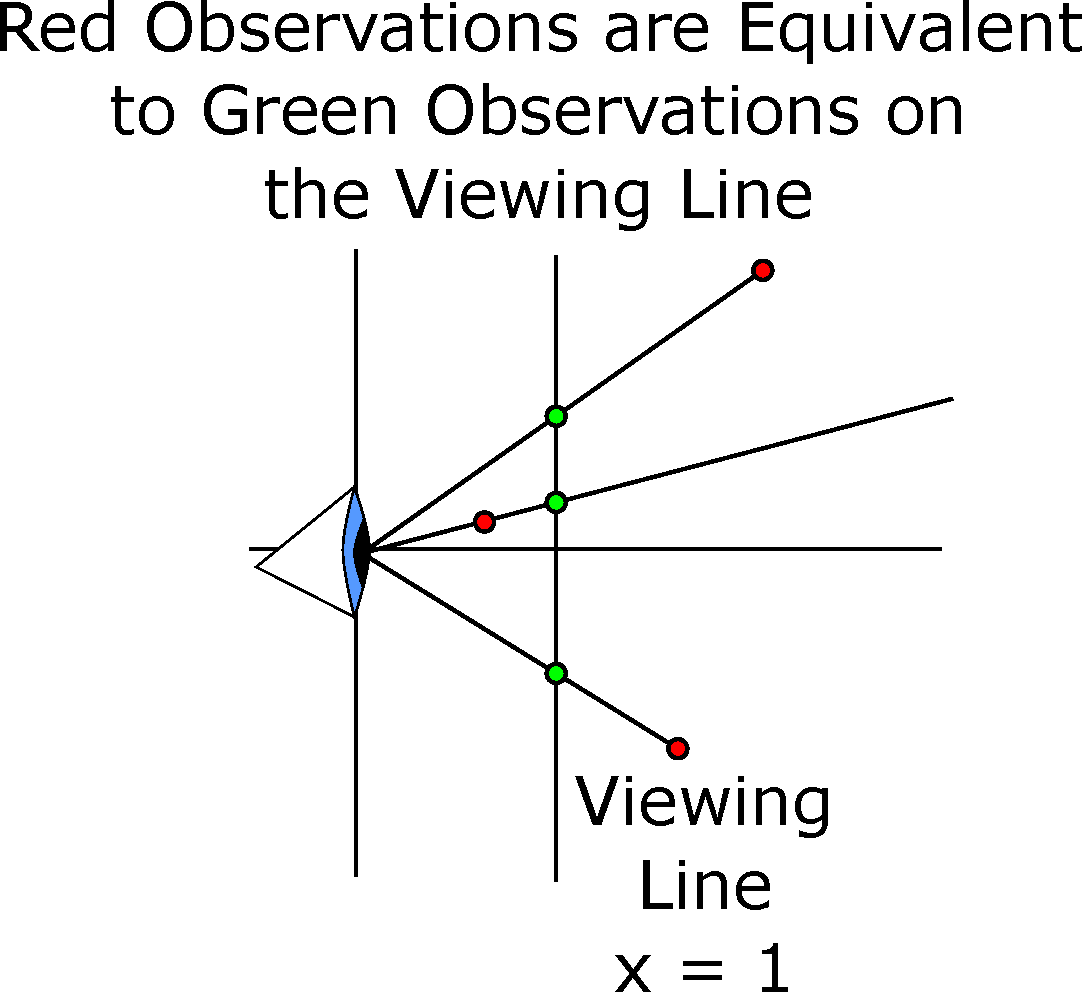
\includegraphics[width = 2in]{oneVarDiffCalc/perspective1.pdf}
\end{figure}

Now imagine that the eye rotates \(\pi/4\) radians counter-clockwise; it is now looking down a line that makes
an angle of \(\pi/4\) radians with the x-axis. Furthermore, its viewing line has rotated to be the 
line \(\left\{y + x = 2\sqrt{\frac{1}{2}} \right\}\). Let \(\tilde y\) denote the position along this 
new viewing line. See the figure below

\begin{figure}[h]
\centering
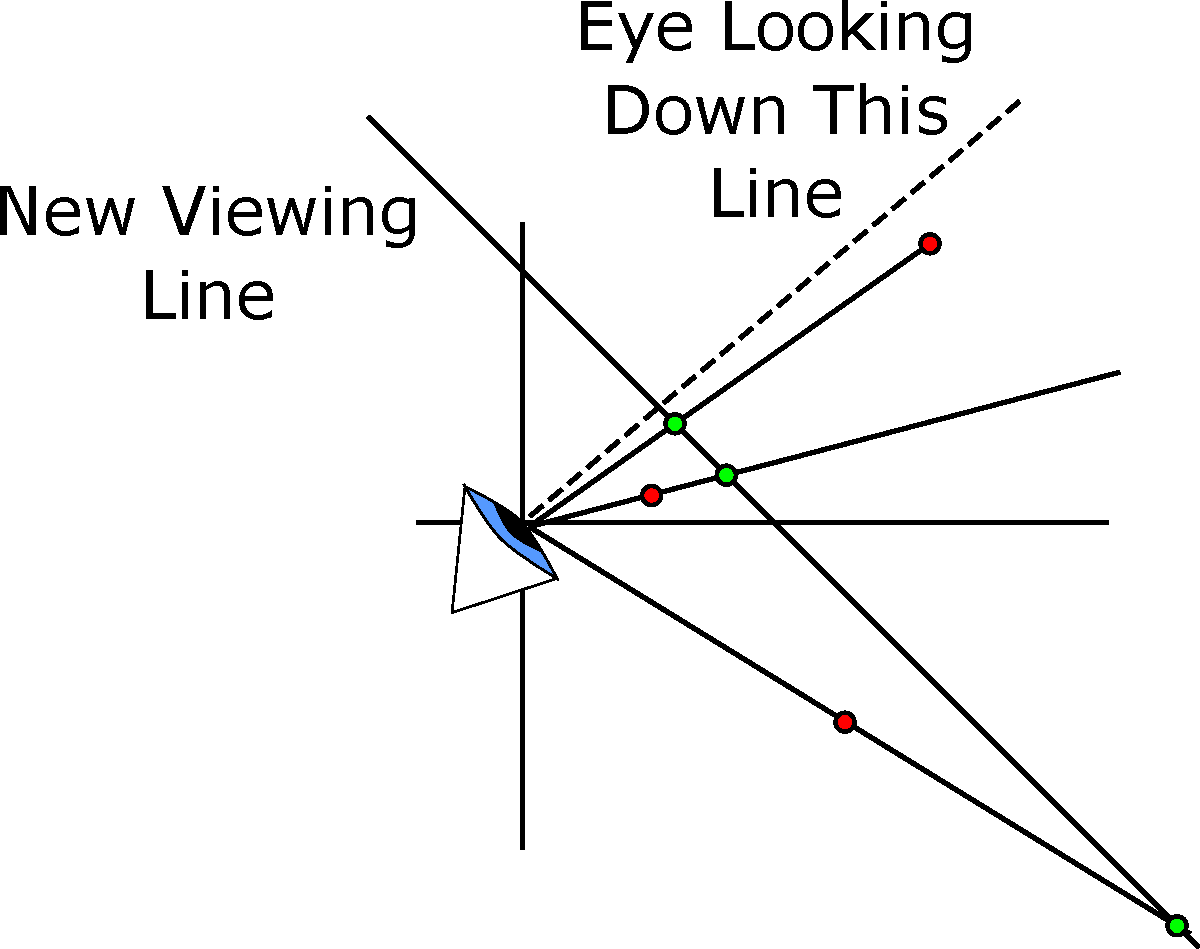
\includegraphics[width = 2in]{oneVarDiffCalc/perspective2.pdf}
\end{figure}

Let \(\tilde y\) measure position on the viewing line relative the line \(\{y = x\}\), i.e. the line that eye is
looking down. If an object appears to be at a point \(y\) on the original viewing line, what is its new position \(\tilde y\) on 
the new viewing line?
The answer turns out to be a linear fractional transformation, i.e.
\begin{equation}
\tilde y = \frac{A + By}{C + Dy},
\end{equation} 
for some constants \(A, B, C,\) and \(D\) depending on the angle of rotation.

Linear fractional transformations are also a classical topic in complex analysis, projective geometry, and
conformal geometry.

\subsubsection*{Finding the Schwarzian Derivative}

Now we will discuss our method of finding the Schwarzian derivative \(Su\) of a function \(u: \mathbb R \to 
\mathbb R\). We will demand that \(Su\) has the following properties:

\begin{enumerate}
\item The Schwarzian derivative is defined by
\begin{equation}
Su = F(u, u', u'', u'''),
\end{equation}
for some function \(F(a, b, c, d)\).

\item Given any function \(u(x)\) and linear fractional transformation \(T(y) = \frac{A + By}{C + Dy}\), we have
that the function defined by
\begin{equation}
w(x) = T(u(x)) = \frac{A + Bu(x)} {C + Du(x)},
\end{equation}
satisfies \(Sw = Su\).
\end{enumerate}

You can interpret the Schwarz derivative via perpective transformations. Suppose there is a particle moving in a
2-dimensional plane and the eye from our first set-up in the previous section observes it at position \(u(t)\)
in its viewing line. Next, suppose another observer is at 45 degrees relative to the first observer (so the 
second set-up) and observes the particle at position \(w(t)\) on their viewing line. Furthermore, suppose
neither observer knows the distance of their viewing plane and doesn't know the angle difference of
their perspectives. Is there some measure of the rate of change in the particle's position that they can agree on?

Yes, the Schwarzian derivative. Their observations differ by some linear fractional transformation; 
since they are missing data on their perspectives, they can't reconstruct the actual position of the particle
and they also can not reconstruct the details of the linear fractional transformation that relates their observations.
However, the Schwarzian derivative will always be the same despite no knowing the exact transformation. It is
enough to just know that it is a linear fractional transformation. 

\subsubsection*{The Problem}

Given the two properties of the Schwarzian derivative listed above, show that
\begin{equation}
F(u, u', u'', u''') = J\left( \frac{u'''}{u'} - \frac{3}{2} \left(\frac{u''}{u'}\right)^2 \right),
\end{equation}
for some function \(J\). Thus, deduce that a reasonable definition of the Schwarzian derivative is
\begin{equation}
Su = \frac{u'''}{u'} - \frac{3}{2}\left( \frac{u''}{u'} \right)^2.
\end{equation} 

\subsubsection*{The Solution}

First, we start by looking at the consequences of having an invariant for translations \(T(y) = A + y\) which
are fractional transformations for \(B = 1, C = 1,\) and \(D = 0\). Note that the derivatives of \(u\) and \(w\)
are equal. So we get that for any function \(u\) that
\begin{equation}
F(u + A, u', u'', u''') = F(u, u', u'', u''').
\end{equation}
Now, note that for any point \((a, b, c, d)\), we can find a function \(u\) such that 
\((u, u', u'', u''') = (a,b,c,d)\) for some point \(x\). So we get that
\begin{equation}
F(a + A, b, c, d) = F(a, b, c, d),
\end{equation} 
for any \(A, a, b, c,\) and \(d\). In particular, since we can vary \(A\) without changing the right
hand side, we see that the value \(F(a, b, c, d)\) is actually independent of \(a\). Therefore, we
may find a function \(G(b, c, d)\) such that
\begin{equation}
F(a, b, c, d) = G(b, c, d).
\end{equation}
Note that \(G(u', u'', u''')\) will be invariant for linear fractional transformations of \(u\) and 
that \(G(u', u'', u''')\) depends only on the derivatives of \(u\).

Next, we consider the effect of scalings \(T(y) = By\), these are also a specific class of linear fractional
transformations. We have that
\begin{equation}
G(Bu', Bu'', Bu''') = G(u', u'', u'''),
\end{equation}
for any \(B\). Similar to before, we get that
\begin{equation}
G(Bb, Bc, Bd) = G(b, c, d),
\end{equation}
for any \(B, b, c,\) and \(d\). Therefore, we see that \(G\) must be homogeneous of degree 0, i.e.
\begin{equation}
G(\lambda b, \lambda c, \lambda d) = G(b, c, d),
\end{equation}
for any constant scaling \(\lambda\).

Next, we consider the specific linear fractional transformation \(T(y) = \frac{1}{y}\). We then have that
\begin{align}
w & = \frac{1}{u}, \\
w' & = -\frac{u'}{u^2}, \\
w'' & = \frac{2u'^2}{u^3} - \frac{u''}{u^2}, \\
w''' & = \frac{6u'u''}{u^3} - \frac{6u'^3}{u^4} - \frac{u'''}{u^2}. 
\end{align}
So from the invariance of \(G\), we get that
\begin{equation}
G(u', u'', u''') = G\left( -\frac{u'}{u^2},
    \frac{2u'^2}{u^3} - \frac{u''}{u^2},
    \frac{6u'u''}{u^3} - \frac{6u'^3}{u^4} - \frac{u'''}{u^2} \right). 
\end{equation}
Now use the 0-homoegeneity of \(G\) to get
\begin{equation}
G(u', u'', u''') = G\left(-1, 
    \frac{2u'}{u} - \frac{u''}{u'}, 
    \frac{6u''}{u} - \frac{6u'^2}{u^2} - \frac{u'''}{u'}\right)
\end{equation}
Note that the expression on the right hand side contains terms involving \(u\) without any derivatives,
which isn't directly supplied as an argument to \(G\) on the left hand side. So when like before we
pass to general coordinates, the \(u\) terms turn into general constants \(A\). So we get
\begin{equation}
G(b, c, d) = G\left(-1, 
    \frac{2b}{A} - \frac{c}{b}, 
    \frac{6c}{A} - \frac{6b^2}{A^2} - \frac{d}{b}\right),
\end{equation} 
for any constant \(A\). So there exists a function \(H\) such that
\begin{equation}
G(b, c, d) = H\left(
    \frac{2b}{A} - \frac{c}{b}, 
    \frac{6c}{A} - \frac{6b^2}{A^2} - \frac{d}{b}\right),
\end{equation}
for any constant \(A\).

The fact that \(A\) is any general constant that appears on the right hand side but is not on the left means that 
there is more information to draw from \(H\). Let \(\theta = \frac{2b}{A} - \frac{c}{b}\). So
\begin{align}
\frac{6c}{A} - \frac{6b^2}{A^2} - \frac{d}{b} & = 
    \frac{3c}{b}\left(\theta + \frac{c}{b}\right)
    - \frac{3}{2}\left(\theta + \frac{c}{b}\right)^2 - \frac{d}{b}, \\
& = 3\left(\theta + \frac{c}{b}\right)\left(\frac{c}{2b} - \frac{\theta}{2}\right) - \frac{d}{b}, \\
& = \frac{3}{2}\left(\frac{c^2}{b^2} - \theta^2\right) - \frac{d}{b}.
\end{align}

So, we get that
\begin{equation}
G(b,c, d) = H\left(\theta, \frac{3}{2}\left(\frac{c^2}{b^2} - \theta^2\right) - \frac{d}{b} \right).
\end{equation}
Now, freeze \(b, c\) and \(d\) while varying \(A\). The left hand side is constant, but the value of \(\theta\)
on the right hand side is varying. So we see that the right hand side is constant on \(\{\theta < -\frac{c}{b}\}\) 
and it is also constant on \(\{\theta > -\frac{c}{b}\}\). Note as long as \(c \neq 0\) and \(b \neq 0\), we can
find a value of \(A\) such that \(\theta = 0\). So we have
\begin{equation}
G(b, c, d) = H\left(0, \frac{3}{2}\left(\frac{c}{b}\right)^2 - \frac{d}{b}\right),
\end{equation}
as long as \(c \neq 0\) and \(b \neq 0\).

So for \(b, c\neq 0\), we can write
\begin{equation}
G(b,c, d) = J\left(\frac{d}{b} - \frac{3}{2}\left(\frac{c}{b}\right)^2 \right).
\end{equation} 
As long as \(J\) is continuous, it extends to \(b \neq0\). So putting it all together, we get
\begin{equation}
F(u, u', u'', u''') = J\left( \frac{u'''}{u'} - \frac{3}{2}\left(\frac{u''}{u'}\right)^2 \right).
\end{equation}
We may take the expression inside parenthesese on the right hand side to be the Schwarzian derivative, i.e.
\begin{equation}
Su = \frac{u'''}{u'} - \frac{3}{2} \left(\frac{u''}{u'}\right)^2.
\end{equation}
You can now directly verify that if \(w(x) = T(u(x))\) for a linear fractional transformation \(T\), then
\(Sw = Su\).
